%!TEX root = ../main.tex

\section*{GCP Titan (TPM)}
\addcontentsline{toc}{section}{GCP Titan (TPM)}

All of Google Cloud runs on Google purpose built servers 
which contain a by google custom build chip, called Titan. 

"Google's purpose-built chip to establish hardware root of trust 
for both machines peripherals on cloud infrastructure" - 
\cite{holzle_bolstering_2017}

According to Google,
 “Titan works to ensure that a machine boots from a known good state 
 using verifiable code, and establishes the hardware root of trust 
 for cryptographic operations in our data centers.” 
 Titan is a Trusted Platform Module (TPM).

At a high level, the Titan chip’s primary duties are to:
Ensure authenticated software components (Secure Boot)
Establish a hardware root of trust (Machine Identity)

\begin{figure}[!ht]
    \centering
    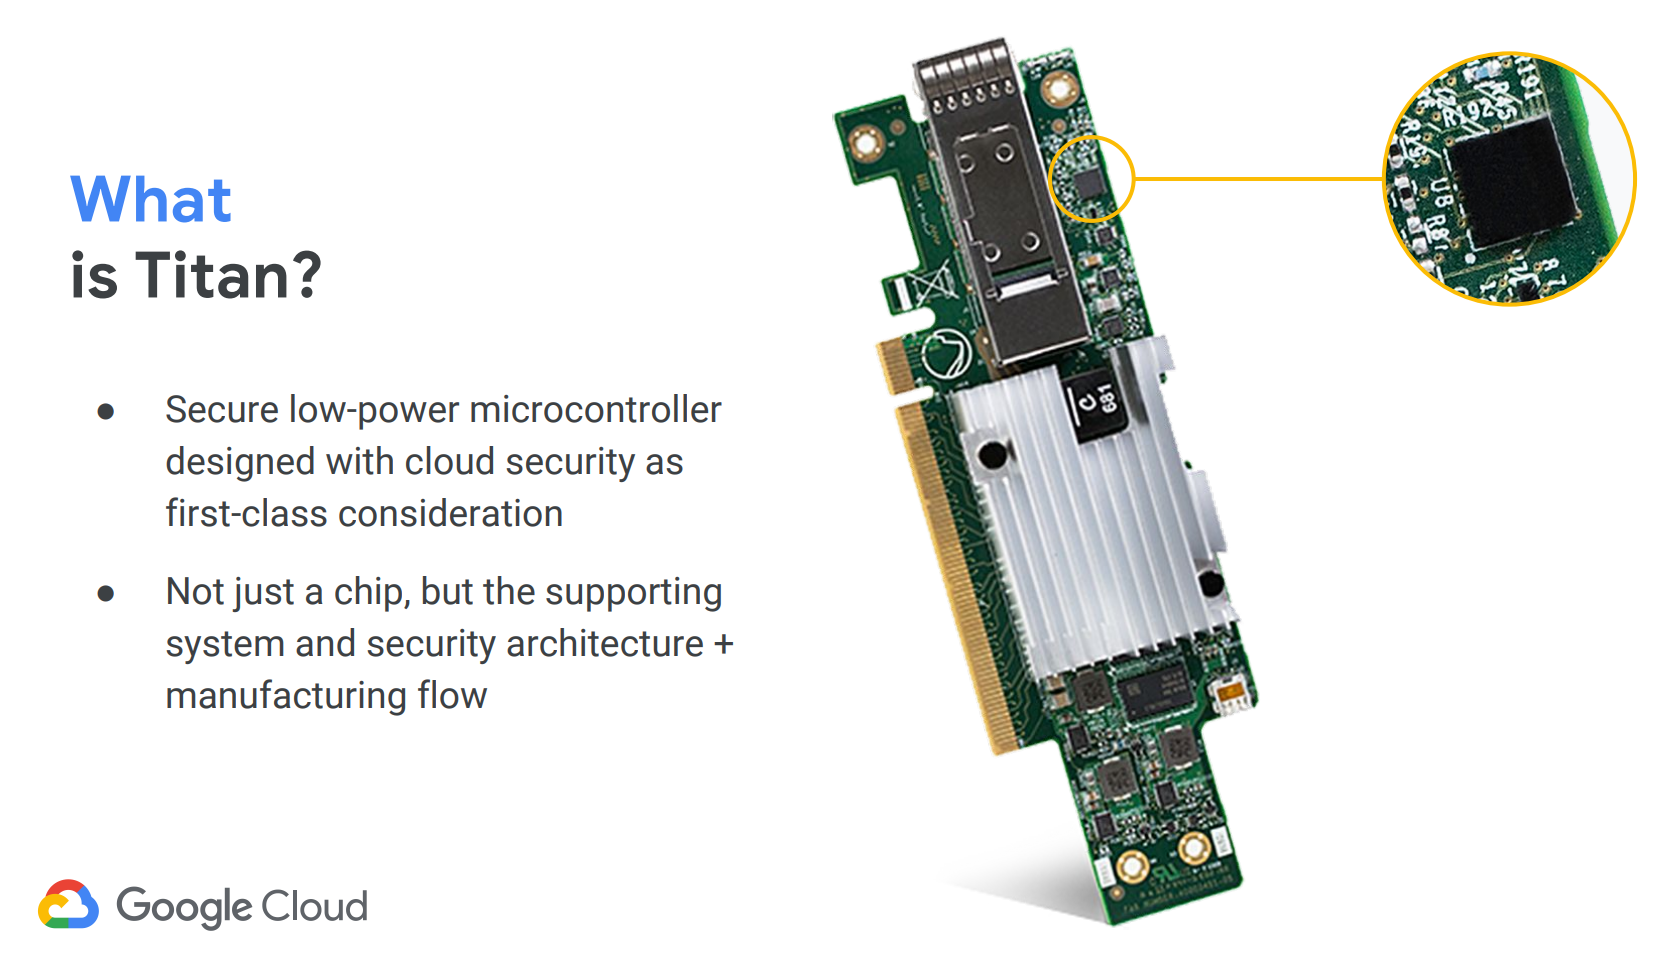
\includegraphics[width=0.5\linewidth]{what-is-titan}
    \caption{What is Titan image from \cite{johnson_titan_2018}}
    \label{fig:what-is-titan}
\end{figure}

Let's explore how Titan performs these duties:

\subsection*{Secure Boot}
Using public key cryptography, 
the Titan chip validates the boot firmware from a known baseline using digital signatures. 
This ensures nothing at the firmware level has been tampered with, and the machine is trusted.

\subsection*{Machine Identity}
Cryptographic keys are fused into the Titan chip during its creation. 
Using these fused keys and cryptography we can ensure the Titan chip is valid, 
creating a hardware base root of trust with which we can establish a trusted identity from.

For a much more in-depth technical explanation of these concepts, 
see this 
blog\footnote{\url{https://cloud.google.com/blog/products/gcp/titan-in-depth-security-in-plaintext} \cite{savagaonkar_titan_2017}} 
from Google on Titan, 
this presentation by Johnson at the secure enclave workshop at google \citep{johnson_titan_2018}, and this ebook on Secure boot \citep{yao_understanding_2021}.

\begin{figure}[!ht]
    \centering
    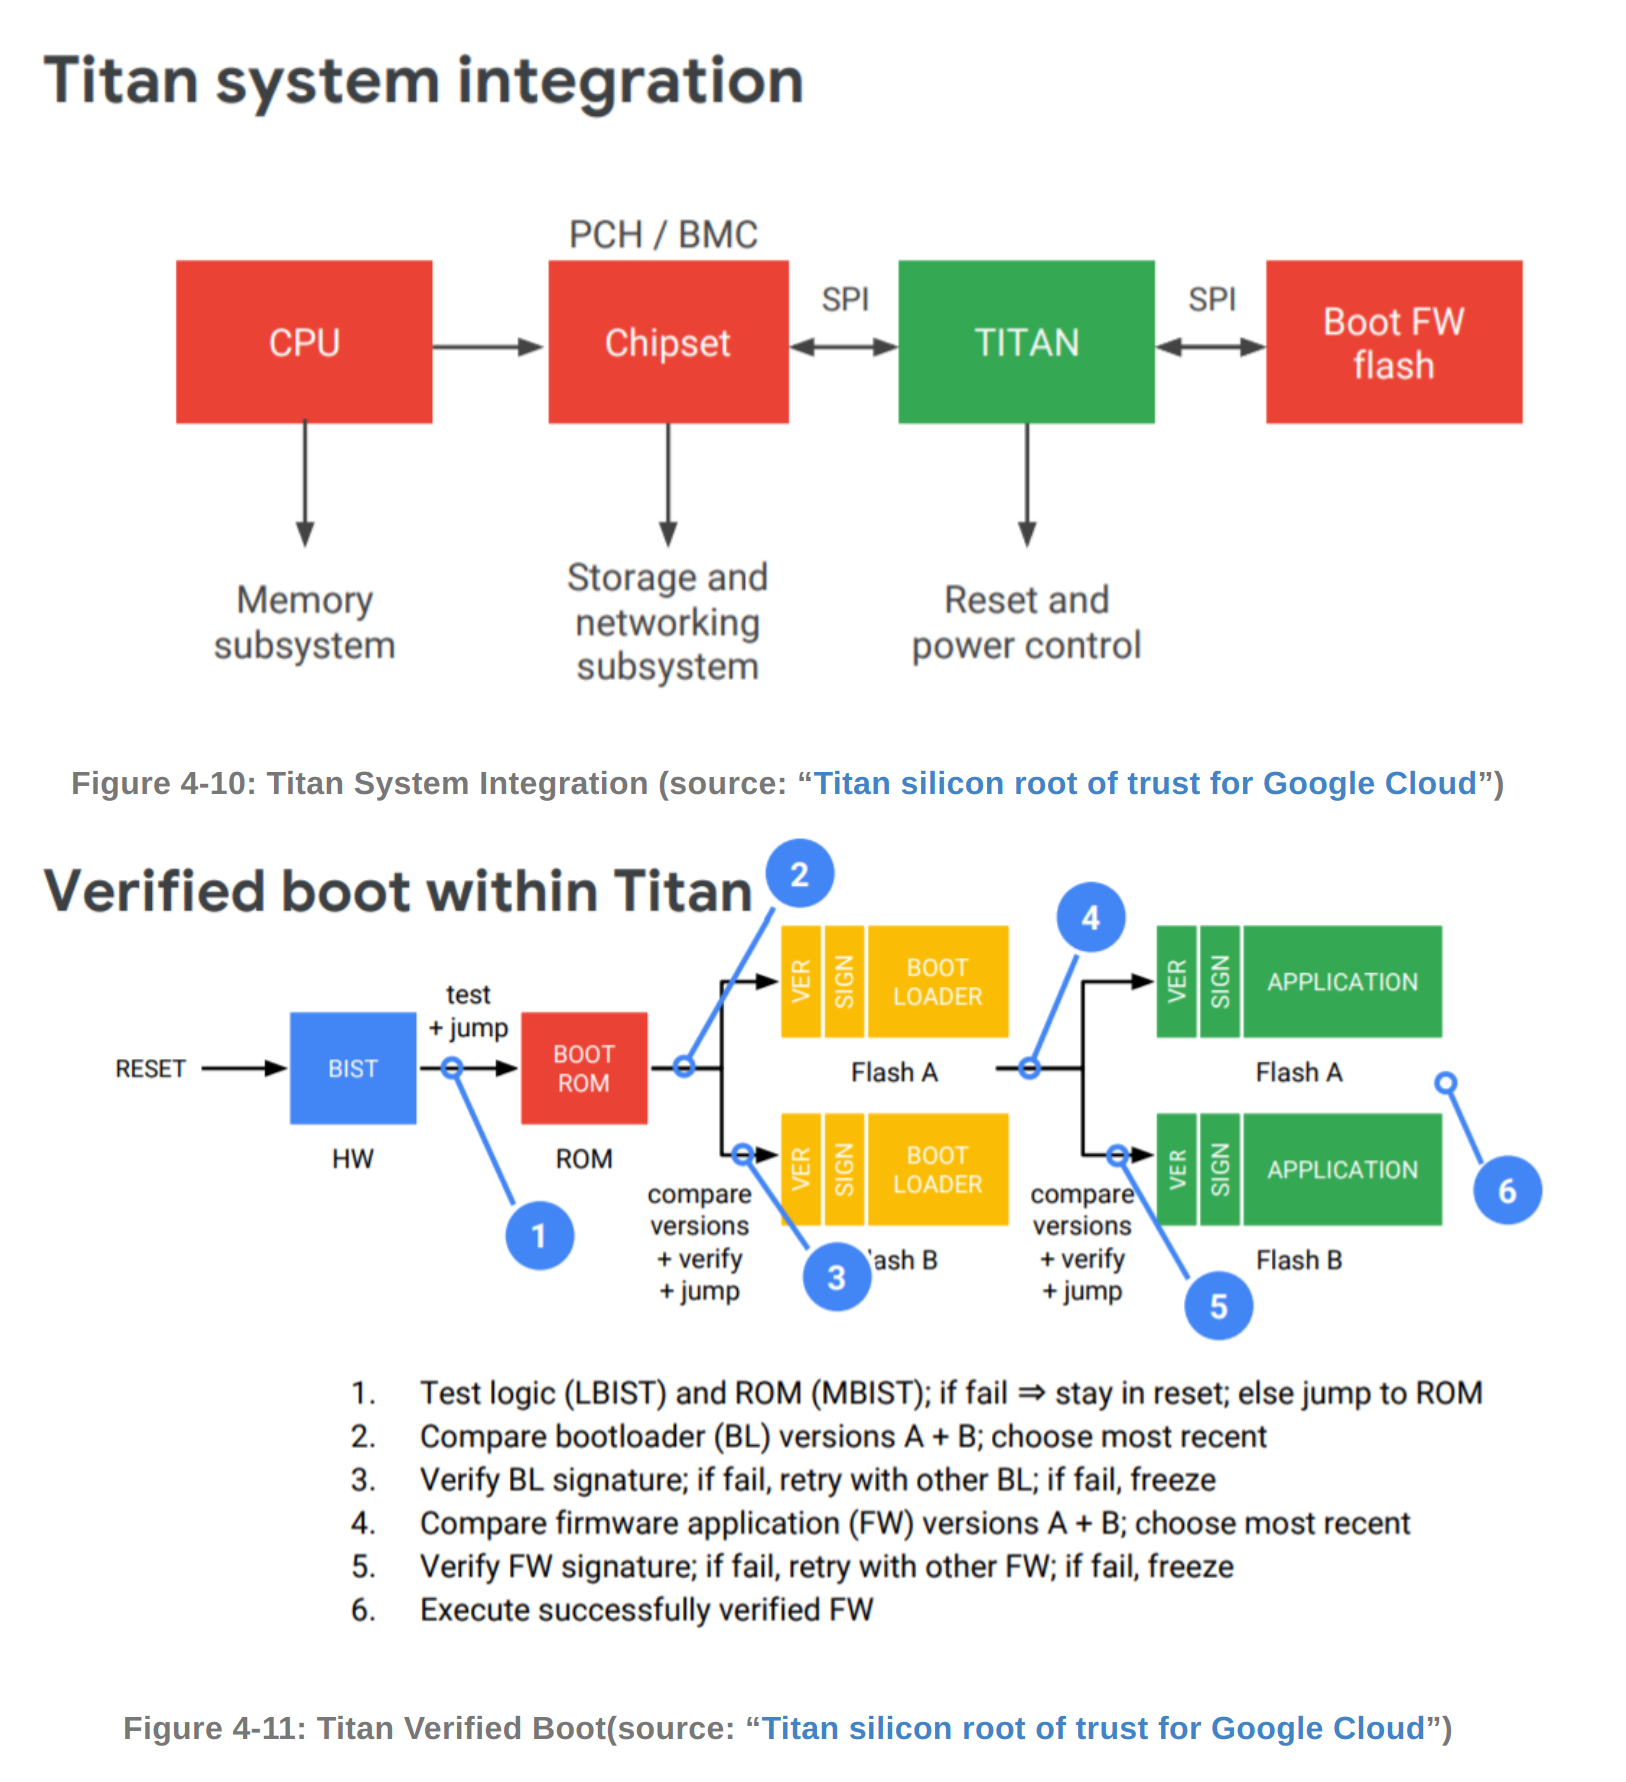
\includegraphics[width=0.5\linewidth]{titan-system-integration}
    \caption{Titan system integration image from \cite{yao_understanding_2021}}
    \label{fig:titan-system-integration}
\end{figure}


\subsection*{Titan extended to Shielded VM’s}
The hardware integrity provided by the Titan chip is extended 
to the Virtual Machine (VM), by the concept of the Shielded VM \citep{leibl_gcp_2022}.

